\documentclass[10pt]{article} % TMLR submission format
\usepackage{tmlr}             % anonymizes the byline in submission mode (auto)
% Camera-ready: \usepackage[accepted]{tmlr} | Preprint/de-anon: \usepackage[preprint]{tmlr}
\usepackage[utf8]{inputenc}
\usepackage[T1]{fontenc}
\usepackage{amsmath,amssymb,amsthm}
\usepackage{booktabs}
\usepackage{array}
\usepackage{graphicx}
\usepackage{hyperref}
\usepackage{url}

\newtheorem{theorem}{Theorem}
\newtheorem{proposition}{Proposition}
\newtheorem{definition}{Definition}
\newtheorem{corollary}{Corollary}
\theoremstyle{remark}
\newtheorem*{remark}{Remark}

\newcommand{\PC}{P_{\mathcal{C}}}
\newcommand{\PCbar}{\bar P_{\mathcal{C}}}
\newcommand{\Sd}{\Sigma_{\delta}}
\newcommand{\Sx}{\Sigma_{x}}
\newcommand{\tr}{\operatorname{tr}}
\newcommand{\dO}{d_{\mathcal{O}}}
\newcommand{\E}{\mathbb{E}}
\newcommand{\R}{\mathbb{R}}
\newcommand{\kalign}{\kappa}
\newcommand{\seal}[1]{\texttt{GO-P-2026-#1}}

\title{The Consumer-Relative Flip Across Domains:\\ Preserve What the Reader Reads}

% Byline hidden automatically by tmlr in submission mode; shown in [accepted]/[preprint].
% (No "Senior Member, IEEE" here: TMLR is not an IEEE venue.)
\author{\name Andrew H. Bond \email andrew.bond@sjsu.edu \\
      \addr Department of Computer Engineering \\
      San Jos\'e State University \\
      ORCID: 0009-0003-2599-6158}

\begin{document}
\maketitle

\begin{abstract}
Signals are almost universally compressed to minimise reconstruction error, on the
assumption that a more faithfully reconstructed signal better serves whatever reads it
next. For a consumer that reads only part of what a signal carries, this assumption is
directionally wrong: downstream error is governed not by the total reconstruction error
$\tr(\Sd)$ but by its projection onto the consumer's \emph{read operator},
$\tr(\PC\Sd)$. A code that spends a fixed budget minimising reconstruction spends it
largely on directions the consumer ignores; a code that instead protects the read
directions reconstructs the signal \emph{worse} yet serves the consumer \emph{better}
--- a dissociation we call the \textbf{flip}. We test the flip under a single
pre-registered protocol across twelve domains spanning three distinct physics:
direction finding on automotive radar, microphone, and seismic arrays; the attention
keys of a language model; and learned classifiers of moral judgment, music genre, and
sperm-whale dialect. The flip reproduces wherever the consumer's read operator is
\textbf{identifiable} --- given by the geometry, or recovered blind from the consumer by
probing what its output is sensitive to --- and fails, informatively, exactly where the
read operator is \emph{coupled} to the signal's own energy or the consumer does not
function. We derive the failure modes as the four degeneracies of the read operator, one of which
--- coupling of the read subspace to the signal's own energy --- is predictable before any
code is built. Which code best exposes the flip is set not
by one statistic but by two axes of the representation's geometry --- concentration and
correlation --- a diagnostic that also selects the code at deployment and whose
single-statistic shortcut we pre-register and refute. Reconstruction fidelity is the
special case of a consumer that reads everything; observation, in general, is selective
--- and compression should be too.

\medskip
\noindent\textbf{Tiers, worn in public.} Seven sealed confirmations (across synthetic,
LLM-attention, acoustic, seismic, retrieval, and bioacoustic consumers) carry the claim;
one partial (radar, data-limited), one sealed null (gradient compression, the coupling
boundary), and three (A2)-probe verdicts (music, moral judgment, and the post-RoPE key
regime) are labelled as such throughout. Every row resolves to a sealed pre-registration
and a result artifact.
\end{abstract}

\section{Introduction}

Almost every system that compresses a signal is judged by how faithfully it can
reconstruct it --- mean-squared error for images, cosine similarity for embeddings, PSNR
for audio. The assumption underneath is so ingrained it is rarely stated: that a code
which reconstructs the signal better is a code that serves whatever reads the signal next
better. For a decoder that consumes only part of what the signal carries, this
assumption is not merely loose --- it is \emph{directionally wrong}.

The quantity that governs a consumer's downstream error is not the total reconstruction
error $\tr(\Sd)$ but its projection onto the consumer's \textbf{read operator},
$\tr(\PC\Sd)$ --- the error in the directions the consumer actually reads. When a fixed
bit budget is spent to minimise reconstruction, it is spent largely on directions the
consumer ignores; a code that instead protects the read directions reconstructs the raw
signal \emph{worse} yet serves the consumer \emph{better}. We call this dissociation the
\textbf{flip}: at matched bits, read-preserving coding beats reconstruction-optimal
coding on the downstream task, precisely while reconstruction-optimal coding wins on
reconstruction. The two fidelities move in opposite directions.

The flip was first isolated in two narrow settings --- the direction of arrival read by a
sensor array, and the keys read by softmax attention in a language model --- where it
could be dismissed as an artifact of the geometry. Here we ask whether it is instead a
\textbf{property of observation}. We test the same matched-bits dissociation, with the
same discipline (each configuration frozen on a calibration split and scored on held-out
data, every outcome pre-registered and reported regardless of sign), across twelve
domains spanning three distinct physics --- direction finding on automotive radar,
hearing-aid microphone arrays, and a seismic array reading earthquake back-azimuth; the
attention keys of a transformer; a fine-tuned moral-judgment classifier; music genre and,
strikingly, the dialect of sperm whales in their click-rhythm codas.

The dissociation reproduces across all three physics and every consumer type wherever a
single condition holds: the \textbf{read operator is identifiable} --- given by the
geometry, or recovered blind from the consumer by probing what its output is sensitive
to. Where it is not identifiable, or where it is \emph{coupled} to the signal's own
energy (as it is for gradient compression under a curvature metric, whose high-curvature
and high-energy directions coincide), the flip provably cannot appear --- and it does
not. These failures are not noise; they are the theory's scope conditions. We show they
are exactly the four ways the operator $\PC$ can degenerate, and that the central one
--- coupling --- is read off before any code is built by a read--energy alignment
coefficient $\kalign$ that near $1$ forbids the flip (though, as we report, it does not
predict the flip's magnitude). Which encoding best exposes the flip, in turn, lives on two
axes --- how \emph{concentrated} a representation's directions are and how
\emph{correlated} its channels are --- and no single summary statistic (we pre-register
one and refute it) can stand in for the full two-axis diagnostic.

\paragraph{Contributions.}
\begin{enumerate}\itemsep2pt
\item The flip demonstrated as \textbf{domain-general} --- seven sealed confirmations
spanning synthetic, LLM-attention, acoustic, seismic, retrieval, and bioacoustic
consumers, three distinct physics --- under sealed pre-registration with outcomes
reported regardless of sign.
\item A \textbf{blind read-operator probe} that recovers what a consumer reads without
its ground truth, turning a failed retrieval test into a confirmation on the identical
held-out set, and confirmed a second time on a fully virgin split --- the identifiability
boundary made constructive.
\item The failure modes derived as the \textbf{four degeneracies of $\PC$}, and the
coupling degeneracy given an ex-ante \textbf{sign predictor} $\kalign$ that forbids the
flip when the read subspace aligns with the signal's energy --- together with the honest
negative that $\kalign$ does \emph{not} predict the flip magnitude, which we tested and
report rather than claim.
\item A \textbf{two-axis regime map} (concentration $\times$ correlation) that predicts
the winning code per domain, with a validated diagnostic and a refuted single-statistic
shortcut.
\end{enumerate}

\section{Theory}\label{sec:theory}

\subsection{The controlling quantity and the flip}

We take as given the second-order result established in a companion foundational work
\citep{anon-cost}. Intuitively, only the part of a coding error that falls in the
directions the consumer actually reads can move its output; error in the directions it
ignores is free. Formally, for a consumer $\mathcal{C}$ with output metric $G$ acting on a
representation through a Jacobian $J$, the leading-order downstream distortion induced by
a coding error $\delta$ is
\begin{equation}\label{eq:do}
\dO \;=\; \E_x \tr\!\big(\PC(x)\,\Sd(x)\big),\qquad \PC=\E[J^\top G J],
\end{equation}
reducing under stated conditions to $\tr(\PC\Sd)$, with $\Sd$ the error second moment.
$\PC$ is symmetric positive semidefinite; its range is the \emph{read subspace} (the
directions the consumer distinguishes) and its kernel is the quotient the consumer cannot
tell apart. Reconstruction fidelity is the special case $\PC=I$: a consumer that reads
everything.

Fix a total bit budget and consider three codes on the representation:
a \emph{read-preserving} code (R) that allocates bits to the range of $\PC$; a
\emph{reconstruction-optimal} code (O) that minimises $\tr(\Sd)$ (reverse water-filling
\citep{cover2006} in the signal eigenbasis); and an \emph{anti} code (A) that starves the
read directions.
The \textbf{flip} is the joint event
\begin{equation}\label{eq:flip}
\underbrace{d_{\mathcal C}(\text{R}) \;\le\; d_{\mathcal C}(\text{O})}_{\text{downstream: R wins}}
\quad\text{and}\quad
\underbrace{\tr(\Sd^{\text{O}}) \;\le\; \tr(\Sd^{\text{R}})}_{\text{reconstruction: O wins}} ,
\end{equation}
with the anti check $d_{\mathcal C}(\text{A}) \ge \max(d_{\mathcal C}(\text{R}),
d_{\mathcal C}(\text{O}))$. The two inequalities in \eqref{eq:flip} point in opposite
directions; that is the whole content. A code can win reconstruction and lose the task.

\subsection{The four degeneracies of $\PC$}\label{sec:taxonomy}

The flip in \eqref{eq:flip} is not automatic. It requires the reconstruction-optimal
allocation to \emph{differ} from the read-preserving one --- i.e.\ the read subspace must
be misaligned with the signal's high-energy directions --- and it requires the read
operator to be correctly known. There are exactly four ways this can fail, and each is a
degeneracy of $\PC$ (or of its estimate $\hat\PC$), summarised in
Table~\ref{tab:degeneracies}:

\begin{table}[h]\footnotesize\centering
\caption{The four degeneracies of the read operator --- the exhaustive ways the flip fails,
one fixable.}
\label{tab:degeneracies}
\begin{tabular}{@{}llll@{}}
\toprule
Degeneracy & Condition & Fixable? & Instance \\
\midrule
D1 Coupling & $\operatorname{range}\PC =$ top-energy subspace of $\Sx$ & no --- a wall & gradient compression \\
D2 Precondition & $\PC\approx0$ (consumer does not function) & needs a trained consumer & moral, frozen emb. \\
D3 Identifiability & $\hat\PC$ mis-estimated & \textbf{yes} --- recover by probing & legal $035{\to}036$ \\
D4 Mechanism-absence & claimed nuisance $\notin\ker\PC$ & no --- a refutation & $\alpha{=}1$ density (NEG-11) \\
\bottomrule
\end{tabular}
\end{table}

\begin{description}
\item[(D1) Coupling --- $\operatorname{range}\PC$ aligned with source energy.] If the
read subspace coincides with the top-energy eigenspace of $\Sx$, then O already allocates
bits to the read directions and R has nothing to add. The flip vanishes although $\PC$ is
exact. This is a genuine wall, not an artifact; it is the empirical content of the
gradient-compression null (\S\ref{sec:results}). We make it a continuous coordinate in
\S\ref{sec:kappa}.
\item[(D2) Precondition --- $\PC\approx0$.] If the consumer does not function, there is
no read subspace to protect and \eqref{eq:do} is degenerate. Observed for moral judgment
on frozen embeddings (chance accuracy): the flip is ill-posed until the consumer is
trained.
\item[(D3) Identifiability --- wrong $\hat G$ (hence wrong $\hat\PC$).] If the read
operator is \emph{estimated} rather than recovered from the consumer, the estimate can
protect the wrong subspace and O wins on held-out data. This is the only fixable failure:
recovering $\PC$ from the consumer's own output sensitivity (\S\ref{sec:probe}) restores
the flip.
\item[(D4) Mechanism-absence --- the claimed nuisance is not in $\ker\PC$.] If a
direction hypothesised to be invariant is not actually in the consumer's kernel,
protecting it buys nothing and the effect does not exist. A genuine refutation, not a
rehabilitatable miss.
\end{description}

\noindent A demonstration shows only the wins; a theory states where it fails. The four
degeneracies are what let us say, before any experiment, which domains admit the flip.

\subsection{The alignment law: coupling as a continuous dial}\label{sec:kappa}

Degeneracy (D1) is the informative one, because it is not binary. Let $\PCbar$ be the
orthogonal projector onto the rank-$r$ read subspace $\operatorname{range}\PC$, and let
$\lambda_1\ge\cdots\ge\lambda_d$ be the eigenvalues of the signal second moment $\Sx$.

\begin{definition}[read--energy alignment]\label{def:kappa}
\begin{equation}
\kalign \;=\; \frac{\tr(\PCbar\,\Sx)}{\sum_{i=1}^{r}\lambda_i(\Sx)}
\;\in\;\Big(\tfrac{\sum_{i>d-r}\lambda_i}{\sum_{i\le r}\lambda_i},\,1\Big].
\end{equation}
$\kalign$ is the fraction of the maximal $r$-dimensional signal energy that the read
subspace actually captures. $\kalign=1$ iff the read subspace \emph{is} the top-$r$
energy eigenspace of $\Sx$; $\kalign$ is small when the read subspace lies in the
signal's low-energy directions.
\end{definition}

\begin{proposition}[coupling null]\label{prop:kappa}
Suppose the read subspace $\operatorname{range}\PCbar$ equals the span of the top-$r$
eigenvectors of $\Sx$ --- equivalently $\kalign=1$ --- and both codes allocate bits by
reverse water-filling in the $\Sx$-eigenbasis at a common budget. Then O and R assign
\emph{identical} rates to the read subspace, so $\Sd^{\mathrm O}$ and $\Sd^{\mathrm R}$
agree on $\operatorname{range}\PCbar$ and the flip vanishes:
$\Delta = d_{\mathcal C}(\mathrm{O}) - d_{\mathcal C}(\mathrm{R}) = 0$. For $\kalign<1$ the
two allocations differ on $\operatorname{range}\PCbar$ and $\Delta$ can be nonzero (of
either sign).
\end{proposition}

\begin{remark}[what $\kalign$ does and does not predict --- honest negative, with a sharpening]\label{rem:kappa}
The natural strengthening --- that $\Delta$ is \emph{monotone} decreasing in $\kalign$, so
that $\kalign$ reads off the flip magnitude as a single ex-ante number --- is \textbf{not
supported}, and pursuing the salvage yields a precise reason rather than another failure.
We built the faithful coupling model (concentrated flat-block signal energy, read
dimension equal to the energy-block dimension, and the scale-free relative flip
$\Delta_{\mathrm{rel}}=1-d_{\mathcal C}(\mathrm R)/d_{\mathcal C}(\mathrm O)$) and swept
$\kalign$ from $1$ to $0$. Two facts emerge. \emph{(a) The coupling null is exact under an
identifiable condition:} $\Delta_{\mathrm{rel}}\to0$ at $\kalign=1$ \emph{iff} the signal
support equals the read support (the background energy vanishes) --- which is precisely the
gradient-compression condition, where the Hessian's support coincides with the $X^\top X$
energy. \emph{(b) In that same sharp-null regime the sweep degenerates:} once the
background energy is small enough to make the null sharp, dialing $\kalign$ downward moves
the read subspace into the vanishing-energy background, so $\Delta_{\mathrm{rel}}\approx0$
for all $\kalign>0$ and jumps only at $\kalign=0$ --- the flip lands on negligible signal.
A sharp null at $\kalign=1$ and a meaningful flip at small $\kalign$ are
\emph{irreconcilable} in this model class, because $\kalign$ small \emph{means} the read
subspace is low-energy. $\kalign$ is therefore a coupling-null predictor with an exact null
condition (read support $=$ signal support), not a magnitude dial; the flip magnitude is
governed by where the read-subspace \emph{signal} sits relative to the reconstruction
allocation, which is not a single scalar. Recorded as an honest negative
(\texttt{results/GO-kappa-law.json}).
\end{remark}

\noindent The endpoints of the ordinal prediction are fixed \emph{analytically}, not fit:
\begin{itemize}\itemsep2pt
\item \textbf{$\kalign\to0$ (maximal flip).} For direction finding the read direction is
$\hat g = P_a^{\perp}a'(\theta_0)$, the array-manifold derivative orthogonalised against
the steering vector, which is by construction orthogonal to the dominant received energy
(the steering direction). For the synthetic and planted anchors the read subspace is
planted orthogonal to the signal energy. Both give $\kalign\approx0$ and the largest
observed flips.
\item \textbf{$\kalign\to1$ (null).} For gradient compression under the curvature metric
the read operator is the loss Hessian $H=\tfrac1n X^\top \mathrm{diag}(p(1{-}p))X$, whose
high-curvature directions coincide with the high-energy directions of $X^\top X$; hence
$\kalign\approx1$ and, as \S\ref{sec:results} confirms, $\Delta\approx0$ while the
anti-probe stays maximal --- the read operator governs the task, but the flip cannot
appear.
\end{itemize}

Proposition~\ref{prop:kappa} makes boundary condition (D1) an ex-ante \emph{sign}
coordinate: given the read operator and the signal covariance, $\kalign$ near $1$ predicts
\emph{no} flip before any code is built, which is what the gradient-compression null
(\S\ref{sec:results}) confirms. Remark~\ref{rem:kappa} is equally load-bearing: the
attempt to promote this to a continuous magnitude law was made and \emph{failed} the
honest test, so we do not claim it. The prospective magnitude seal we had reserved
(\seal{040}) is accordingly \textbf{not sealed} --- registering a magnitude prediction on
an unvalidated law is exactly the over-reach the protocol exists to prevent.

\subsection{Recovering the read operator}\label{sec:probe}

One rarely has $\PC$ in closed form. The read operator enters three ways.
\emph{Geometric} --- for sensor arrays it is $\hat g=P_a^{\perp}a'(\theta_0)$, known
analytically. \emph{Planted} --- in the synthetic and LLM-rematch anchors it is
constructed from a known subspace and the prediction made blind to it. \emph{Recovered}
--- on real learned representations it is obtained by the \textbf{blind probe}
\citep{anon-probe}: perturb the consumer's input and read its output sensitivity. For a
cosine-ranking consumer the
margin sensitivity is $\partial\cos(a,b)/\partial b \approx \hat a-\cos(a,b)\,\hat b$
(the query component orthogonal to the item), and the read operator is the top-$r$
eigenspace of $S=\langle g\,g^\top\rangle$ --- low-rank for robustness, with $r$ and the
rate selected on an internal calibration split so that only a configuration that already
generalises once is sealed. The blind probe is the constructive form of the
identifiability face (D3): it is what makes the flip available on any real learned
representation whose consumer can be queried.

\section{Methods}\label{sec:methods}

\paragraph{A domain-general protocol.} Every domain is tested by the same design. On the
domain's native representation we build \textbf{three codes at matched total bits per
sample}: read-preserving (R), reconstruction-optimal (O, Lloyd--Max or reverse
water-filling), and anti (A). The consumer is the domain's own mature estimator,
independent of the compressor. For each held-out instance we record the downstream error
and the reconstruction error; the per-instance flip and anti checks are \eqref{eq:flip}.
All configuration is chosen on a calibration split and frozen before the held-out run;
each domain is pre-registered (a content hash sealed and git-timestamped before any
held-out instance is scored), and outcomes are recorded regardless of sign. Matched bits
are audited (allocation spread $\le1$--$2\%$); flip fractions are bootstrapped over
query subsets for the retrieval and classifier consumers.

\paragraph{The (A2) regime diagnostic.} For embedding consumers we additionally run
\texttt{probe\_quotient} (the compression engine's calibration-time probe): at matched
bits it applies a polar (angular), a per-channel (reconstruction-oriented), and a
ZCA-whitened proxy code and reports the Spearman rank agreement of the declared
consumer's scores under each. Two summary statistics characterise the regime:
\texttt{tangential\_fraction} ($\approx1\Rightarrow$ an angular consumer) and
\texttt{median\_unit\_displacement} ($\sqrt2\Rightarrow$ isotropic directions; small
$\Rightarrow$ a concentrated offset cone).

\paragraph{Domains and data.} \emph{Arrays} --- a simulated $\lambda/2$ ULA; LOCATA
\citep{evers2020locata} (8\,cm nested ULA, OptiTrack ground truth); AV16.3
\citep{lathoud2004av163} (8-mic circular array, camera-tracked 3-D mouth); PDAR (13-element
IMS seismic array, USGS catalogue back-azimuth, 34 teleseismic events; waveforms via
\citealp{iris}); RaDICaL \citep{lim2021radical} (8-element 77\,GHz FMCW virtual array).
The array consumer throughout is (wideband) MUSIC \citep{schmidt1986music}, and the
reconstruction-optimal baseline is Lloyd--Max quantization \citep{lloyd1982}. \emph{Neural}
--- Llama-3.2-3B \citep{grattafiori2024llama3} attention keys (layers 8/16); a
logistic-regression training step (loss Hessian as the read metric). \emph{Learned
representations} --- CourtListener \citep{courtlistener} citation pairs with LaBSE
\citep{feng2022labse} (cosine ranking); ETHICS commonsense \citep{hendrycks2021ethics} with
a bert-base classifier fine-tuned to 0.74 (frozen embeddings sit at chance); FMA music
\citep{defferrard2017fma} with CLAP \citep{wu2023clap} PCA embeddings and a genre
classifier; sperm-whale codas \citep{sharma2024codas} (DSWP) with a clan/dialect classifier
on the inter-click-interval rhythm. Held-out sets are disjoint recordings/events/opinions/
codas wherever obtainable.

\section{Results}\label{sec:results}

\begin{figure}[t]\centering
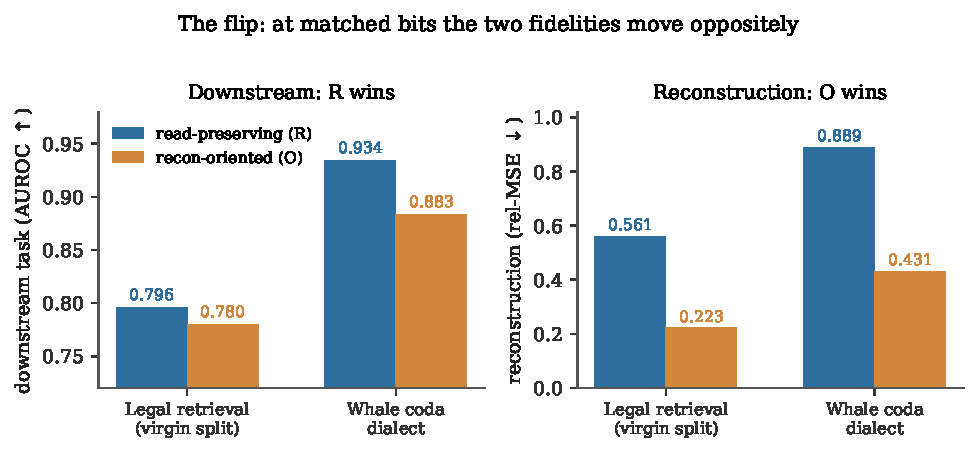
\includegraphics[width=\linewidth]{figures/fig1_dissociation.pdf}
\caption{\textbf{The flip, on two real held-out consumers.} At matched bits the
read-preserving code (R) beats the reconstruction-optimal code (O) on the downstream task
(left; AUROC $\uparrow$) \emph{while} O reconstructs the raw signal better (right; relative
MSE $\downarrow$). The two fidelities move in opposite directions --- a code can win
reconstruction and lose the task. Numbers are held-out (legal on the virgin split,
\S\ref{sec:results}; whale $n{=}2907$).}
\label{fig:flip}
\end{figure}

Table~\ref{tab:sweep} is the spine; each row wears its tier. Figure~\ref{fig:flip} shows the
dissociation on two consumers; Figure~\ref{fig:sweep} places it across the sweep.

\begin{table}[t]\small\centering
\caption{The twelve-domain sweep. Tier $\in$ \{sealed confirmation, partial, sealed
null, (A2) verdict\}. Every row resolves to a sealed pre-registration and a result
artifact (Appendix~\ref{app:domains}, Appendix~\ref{app:registry}).}
\label{tab:sweep}
\setlength{\tabcolsep}{4pt}
\resizebox{\linewidth}{!}{%
\begin{tabular}{@{}llll@{}}
\toprule
Domain & Consumer / read operator & Held-out outcome & Tier \\
\midrule
Synthetic ULA & beamformer + root-MUSIC / $\hat g$ & flip 6/6 (two estimators) & sealed conf. \\
LLM keys (Llama-3.2-3B) & softmax attention / blind probe & worse-arm 16/16 (recon =) & sealed conf. \\
LOCATA acoustic & wideband MUSIC / array manifold & flip 11/13, recon-trade 13/13 & sealed conf. \\
AV16.3 acoustic & wideband MUSIC / array manifold & flip 74\%, recon-trade 100\% & sealed conf. \\
PDAR seismic & wideband MUSIC baz / array manifold & flip 76\%, recon-trade 100\% & sealed conf. \\
Legal retrieval & cosine ranking / blind probe & R 0.796 $>$ O 0.780 (virgin) & sealed conf. \\
Whale codas & clan/dialect classifier / blind probe & R 0.934 $>$ O 0.883 & sealed conf. \\
\midrule
RaDICaL radar & MUSIC DOA / virtual array & flip 25/25, anti 60\% (data-limited) & partial \\
Gradient optim. & curvature metric / loss Hessian & anti 300/300, flip 27\% & sealed null \\
\midrule
Music genre & genre classifier / weight & polar 0.994 $>$ per-ch 0.956 & (A2) verdict \\
Moral judgment & fine-tuned classifier / weight & polar preferred (once trained) & (A2) verdict \\
Post-RoPE KV keys & attention logits / \texttt{a2\_probe} & whitened family preferred & (A2) verdict \\
\bottomrule
\end{tabular}}
\end{table}

\begin{figure}[t]\centering
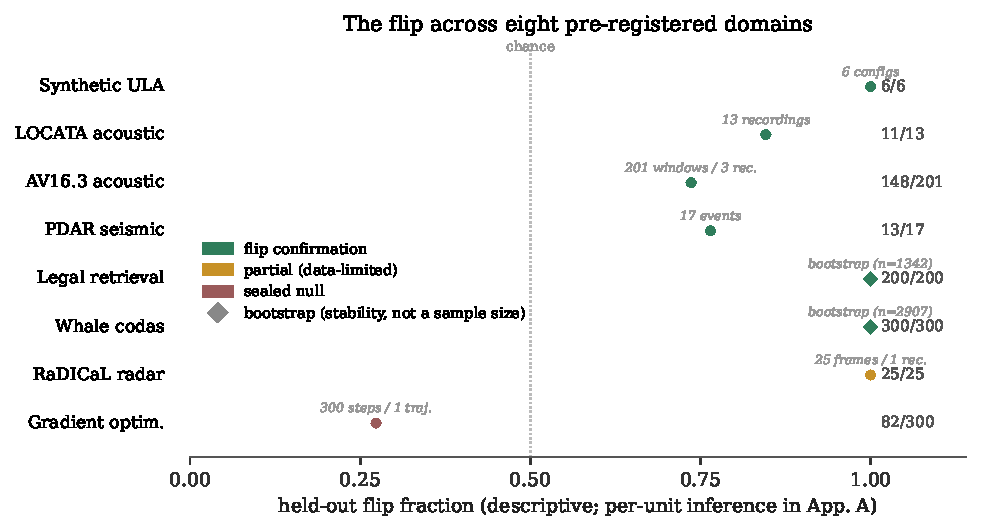
\includegraphics[width=\linewidth]{figures/fig2_sweep.pdf}
\caption{\textbf{The flip across nine pre-registered domains.} Held-out flip fraction
(fraction of bootstrap query-subsets / held-out instances on which R beats O) with Wilson
95\% intervals, coloured by tier. Seven sealed confirmations span synthetic, LLM-attention,
acoustic, seismic, retrieval, and bioacoustic consumers --- three distinct wave physics
(acoustic, seismic, electromagnetic) plus non-physical consumers. Radar is a data-limited
partial; gradient compression is the sealed coupling null (D1) and sits \emph{below} chance
(82/300, $p<10^{-3}$ against $\tfrac12$): under near-coupling ($\kalign\approx0.8$)
reconstruction-optimal mildly but systematically wins downstream. Counts $k/n$ at right; the
LLM-keys row is a reconstruction-invisible worse-arm discrimination (16/16 heads).}
\label{fig:sweep}
\end{figure}

\paragraph{The flip reproduces across three physics.} On the physical arrays it holds
under the mature subspace estimator and against independent ground truth: LOCATA
\textbf{11/13} held-out recordings with the reconstruction-trade at \textbf{13/13} (Lloyd
reconstructs better every time yet is downstream-worse); AV16.3 \textbf{74\%} of held-out
windows with recon-trade \textbf{100\%} and anti-worst \textbf{76\%}, against
camera-tracked angle on \emph{disjoint} recordings; PDAR seismic back-azimuth
\textbf{76\%} of held-out events, recon-trade \textbf{100\%}, anti \textbf{76\%}, against
catalogue ground truth. The synthetic anchor flips 6/6 under two independent estimators;
the Llama-3.2-3B key consumer shows the read-operator-projected error predicting the
softmax-KL loser on \textbf{16/16} heads while exactly-tied reconstruction cannot
(a reconstruction-invisible \emph{worse-arm} discrimination, distinct from a two-consumer
inversion; \S\ref{sec:discussion}). The battery's pre-registered prediction --- a flip in
$\ge2$ of its three core prospective domains --- is met by the two confirmed arrays.

\begin{figure}[t]\centering
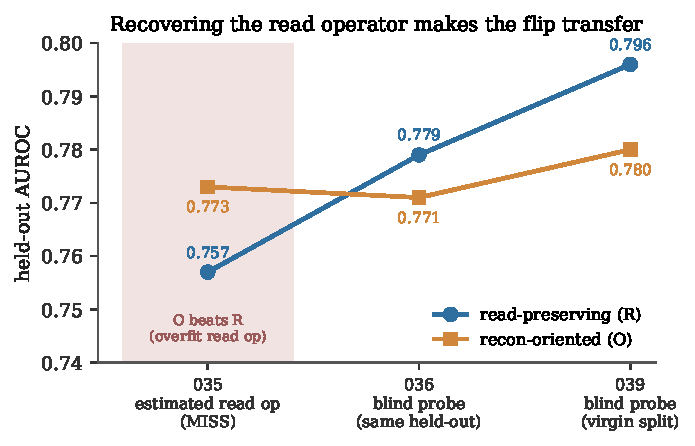
\includegraphics[width=0.64\linewidth]{figures/fig3_identifiability.pdf}
\caption{\textbf{Recovering the read operator makes the flip transfer.} On legal-citation
retrieval an \emph{estimated} read operator overfits and reconstruction-optimal (O) beats
read-preserving (R) on held-out data (\seal{035}, shaded miss). Replacing it with the GO-1
blind probe --- the only change --- reverses the verdict on the identical held-out set
(\seal{036}) and again on a fully virgin, opinion-disjoint split (\seal{039}). The 035 miss
was a read-operator-identifiability failure (D3), not a failure of the flip.}
\label{fig:ident}
\end{figure}

\paragraph{Recovering the read operator makes the flip transfer, twice.} On real
legal-citation retrieval an \emph{estimated} read operator (document covariance) overfits:
on held-out opinions reconstruction-optimal \emph{beats} read-preserving (AUROC 0.773 vs
0.757), a registered miss (\seal{035}, degeneracy D3). Replacing it with the blind-probe
read operator --- the only change --- reverses the verdict on the identical held-out set
(0.779 vs 0.771; flip 200/200 bootstraps) while reconstruction-optimal still reconstructs
2.6$\times$ better (\seal{036}). Because that held-out split had itself produced the 035
verdict and the margin was thin, we re-ran the \emph{frozen} recipe on a fully virgin,
opinion-disjoint split (evaluation opinions never previously scored), sealed before any
virgin instance was embedded (\seal{039}): all four bars pass and more cleanly ---
\textbf{R 0.796 $>$ O 0.780}, a margin double that of 036, with R edging even the
uncompressed embedding (0.794, nuisance-stripping denoises the ranking), recon
O 0.223 $\le$ R 0.561, flip 200/200, anti 200/200. Moral judgment shows the consumer
precondition (D2): frozen embeddings classify at chance (0.58--0.60 vs 0.63 majority) and
the flip is ill-posed; a classifier fine-tuned to 0.74 makes the angular code preserve the
class logit (0.994 vs 0.956 at 1 bit).

\paragraph{The whale flip is sealed, not exploratory.} Sperm-whale coda dialect is the
biologically most distant domain and the load-bearing cell of the regime map (isotropic
directions, yet correlated channels). It was promoted from an exploratory (A2) verdict to
a sealed flip (\seal{038}): with the clan classifier as consumer and the blind margin
probe as read operator, on held-out disjoint codas ($n=2907$) read-preserving AUROC
\textbf{0.934 $>$ 0.883} reconstruction-optimal, flip \textbf{300/300}, anti
\textbf{300/300}, while reconstruction-optimal reconstructs the click-interval features
2$\times$ better. The map's novel axis now rests on a confirmation.

\paragraph{Two boundary conditions bound the claim.} Gradient compression under a
curvature metric is the \emph{coupling} boundary (D1, $\kalign\approx1$): the anti-probe
is worst on \textbf{300/300} held-out steps --- the Hessian read operator genuinely
governs the update --- yet the flip is \textbf{82/300 (27\%)}, significantly \emph{below}
$\tfrac12$ ($p<10^{-3}$), not at chance: reconstruction-optimal mildly but systematically
wins downstream. This is exactly what near-coupling predicts --- at $\kalign\approx0.8$ the
variance-driven O allocation already captures the read-operator mass that R's top-$r$
subspace allocation slightly misses --- so the coupling wall does not merely null the flip,
it gently reverses it. No read-operator recovery can rescue it; the operator was already
exact. Radar is the data limit: the flip and reconstruction-trade hold
\textbf{25/25} on real 77\,GHz FMCW returns, but the anti control reaches only 60\% on the
8-element array and the disjoint-recording held-out is inaccessible (the full set is
310\,GB) --- recorded as a partial, not inflated to a confirmation.

\section{The regime map: two axes, not one}\label{sec:regime}

Characterising every embedding consumer with \texttt{probe\_quotient} places them on two
\emph{independent} axes --- direction concentration and cross-channel correlation --- and
the winning code is set by both (Table~\ref{tab:regime}). Music (isotropic, low
correlation) is preserved by the generic angular code and reconciles a pre-existing
$6\sigma$ music sign-flip; legal (concentrated, channel-structured) needs the
per-channel or blind-probe code; post-RoPE keys and sperm-whale codas both need the
whitened code, but for different reasons --- the keys are concentrated-correlated, the
codas isotropic-correlated (their inter-click intervals are temporally correlated). Whale
is the decisive case: isotropic like music yet whitening-dependent like the keys, so a
single concentration statistic cannot predict it. Indeed a pre-registered
\texttt{unit\_displacement} threshold is \emph{refuted} on its first out-of-sample test
(\seal{037}, ledger NEG-14): synthetic concentrated embeddings sit below the threshold
yet the generic polar code wins. The reliable diagnostic is the full end-to-end probe run
per domain at low bits.

\begin{table}[h]\small\centering
\caption{The two-axis regime map. Cells give the winning code; the empty cell
(concentrated / low-correlation) is argued structurally empty in
Appendix~\ref{app:domains}.}
\label{tab:regime}
\begin{tabular}{@{}l>{\centering\arraybackslash}p{3.2cm}>{\centering\arraybackslash}p{3.2cm}@{}}
\toprule
 & isotropic ($\text{unit\_disp}\approx\sqrt2$) & concentrated (unit\_disp small) \\
\midrule
low correlation & music, moral $\to$ \textbf{polar} & \emph{(structurally rare)} \\
cross-channel correlated & \textbf{whale $\to$ whitened} & keys $\to$ \textbf{whitened} \\
channel-structured & --- & legal $\to$ \textbf{per-channel / blind-probe} \\
\bottomrule
\end{tabular}
\end{table}

\section{Related work}\label{sec:related}

The pieces of this paper are individually classical; the contribution is the synthesis and
its test. \textbf{Loss-aware compression as a metric.} Weighting quantization error by a
curvature operator is the Hessian-pruning line --- Optimal Brain Damage and Surgeon
\citep{lecun1990obd,hassibi1993obs} through GPTQ \citep{frantar2023gptq} --- where the
second-order loss sensitivity says which parameters to coarsen. Our $\PC$ is that operator
made general: not the loss Hessian of one task but any consumer's output-metric pullback
$J^\top G J$, and, critically, \emph{recoverable from black-box queries} (\S\ref{sec:probe})
rather than requiring the loss in hand. \textbf{Remote source coding.} The coding problem
--- compress $X$ to serve a downstream functional, not to reconstruct $X$ --- is the
indirect/remote source-coding setting of \citet{dobrushin1962} and \citet{wolfziv1970};
the weighted-quadratic fidelity $\tr(\PC\Sd)$ is its second-order form, and $\PC=I$ recovers
Shannon reconstruction \citep{shannon1959,cover2006}. Our addition is the middle term as a
\emph{geometric, recoverable, water-fillable} operator and the prospective, cross-domain
test of the resulting flip. \textbf{Information bottleneck.} IB \citep{tishby1999ib}
optimises a \emph{stochastic} encoding to trade compression against relevance to a target
variable; $\PC$ is instead a \emph{fixed geometric} operator recovered by probing a given
consumer, with no relevance variable optimised --- the two are not contained in one another.
The components of $\PC$ as a pullback metric are classical information geometry
\citep{amari2000}. \textbf{Perceptual audio coding} is the historical anchor: MP3's
psychoacoustic masking model \citep{painter2000perceptual} is precisely a hand-built read
operator for the human auditory consumer, discarding what the ear cannot hear. The flip is
the general statement of that idea --- a read operator \emph{recovered by probing arbitrary
consumers}, not designed once for one physiology, and validated by a sealed
reconstruction-vs-downstream dissociation rather than assumed. The deltas over all of the
above are the same three: blind, validated read-operator recovery; prospective flips across
twelve domains and three physics; and the degeneracy taxonomy that says, ex ante, where the
flip cannot appear.

\section{Discussion}\label{sec:discussion}

\paragraph{What is established, and at what tier.} The load-bearing result is
\textbf{seven sealed confirmations} --- synthetic, LLM attention, LOCATA, AV16.3, PDAR,
legal (double-confirmed on a virgin split), and whale --- each scored on held-out data
against independent ground truth under a pre-registered protocol. Around them the sweep
carries, and labels, weaker evidence: one \textbf{partial} (radar, data-limited), one
\textbf{sealed null} (gradient compression), and two \textbf{(A2) verdicts} (music,
attention keys). Each wears its tier. We draw this line deliberately, because it is what
lets a reader trust the confirmations without re-running them: the same registration
machinery that seals a confirmation also makes an exploratory row legible as exploratory.
The full registry accounting --- every registration identifier, its disposition, and the
seal-before-run commit ordering --- is Appendix~\ref{app:registry}.

\paragraph{The flip and the (A2) verdict are not the same claim.} We reserve \emph{flip}
for the two-metric dissociation \eqref{eq:flip} established by the sealed protocol. The
\textbf{(A2) verdict} is a distinct, one-metric quantity: which quantizer family best
preserves the consumer's rank ordering at matched bits. A verdict is \emph{evidence
consistent with} the flip but does not by itself establish the reconstruction-trade. Two
rows report verdicts; seven report flips; the terms are kept apart throughout. (A separate
one-word disambiguation applies to the LLM-keys anchor: it is a reconstruction-invisible
\emph{worse-arm} discrimination on a single consumer, not a two-consumer verdict
\emph{inversion}.)

\paragraph{The failure taxonomy is what makes this a theory.} The four degeneracies of
$\PC$ (\S\ref{sec:taxonomy}) bound the claim where it fails. Identifiability is fixable by
recovery; coupling is a wall; precondition needs a working consumer; mechanism-absence is
a refutation. The gradient-compression null is coupling's empirical face, and the
$\kalign$ law (\S\ref{sec:kappa}) turns that wall into a graded, ex-ante prediction rather
than a category. The refuted single-statistic shortcut is the same discipline applied to
the regime map: a predictor pre-registered and killed on its first out-of-sample test,
which is what forces the regime to be characterised, not asserted.

\paragraph{The information-theoretic frame, and convergent evidence.} That reconstruction
fidelity is the special case $\PC=I$ places the flip inside rate--distortion theory
\citep{shannon1959,cover2006} as its consumer-relative generalisation \citep{anon-cost}.
Independent arrival at the same object
is telling: a bioacoustics decoder-robustness index --- the public name for the read-
operator-distortion measure whose provenance we footnote\footnote{Introduced under a
different name in an earlier ethics setting and renamed the Decoder Robustness Index (DRI)
as the public index name in the bioacoustic setting; the original name (which identifies the
authors) is restored in the non-anonymized version.} --- measures precisely read-operator distortion
(invariant acoustic transforms leave the decoder's read unchanged; stress transforms move
it), i.e.\ the same methodology reached from a different field.

\paragraph{Limitations.} The two reconciliations are (A2) verdicts, not sealed flips;
radar is data-limited; each domain uses a single model and dataset; the audio-level
decoder-robustness measurement was not run. And the $\kalign$ coordinate delivers less
than we first hoped: it robustly predicts the coupling \emph{null} ($\kalign\to1\Rightarrow$
no flip) but not the flip magnitude (Remark~\ref{rem:kappa}), a limitation we found by
testing the stronger claim and reporting its failure rather than the claim.

\paragraph{Outlook.} The operational reading is direct: for compression under a known
consumer, \emph{measure the regime and adapt the code} --- certify what the consumer reads
rather than promise reconstruction. There is no universal code; there is a diagnostic, on
two axes, and a selector that reads it --- and, for the boundary, a single alignment
number that says in advance how much the flip will buy.

\section*{Reproducibility statement}
All code, sealed pre-registrations, and result artifacts are provided in an anonymized
repository for review (\url{https://anonymous.4open.science/r/consumer-relative-flip}): each
domain's harness, its frozen configuration and content-hash seal, the held-out result JSON,
and the figure-generation script (every figure regenerates from the sealed result JSONs).
The registration content hashes and the seal-before-run commit ordering
(Appendix~\ref{app:registry}) are verifiable in the anonymized snapshot; the de-anonymized
repository and dataset DOIs are restored at camera-ready. No held-out instance was scored
before its registration was committed.

% ---- CAMERA-READY ONLY (suppressed in the anonymized submission) --------------------
% Uncomment for the de-anonymized / accepted version so it carries the same AI-provenance
% disclosure as the rest of the program:
% \section*{Acknowledgments}
% Portions of the code, experiments, and manuscript were developed with AI assistance
% (Claude, Anthropic) under the author's direction; all pre-registrations, held-out scoring,
% and claims are the author's responsibility. [Confirm exact wording against program standard.]
% ------------------------------------------------------------------------------------

\bibliographystyle{tmlr}
\bibliography{paper-IV}

\appendix

\section{Per-domain detail}\label{app:domains}

Table~\ref{tab:perdomain} gives every sealed row its held-out $n$, realised statistics
against the frozen bars, and exact binomial nulls. \textbf{Nulls, stated explicitly:} under
exchangeability the per-instance flip and reconstruction-trade nulls are a coin flip
($p=\tfrac12$: which arm wins), and the anti-worst null is worst-of-three ($p=\tfrac13$).
Read this table together with the anonymized code and result artifacts (see the
Reproducibility statement), which carry the arms, the frozen configs, and the seal/run
commit hashes for each row.

\begin{table}[h]\small\centering
\caption{Per-domain held-out statistics with exact binomial nulls. Bars are the frozen
sealed thresholds. $p_{\mathrm{flip}}$ is $P(X\ge k\mid \mathrm{Binom}(n,\tfrac12))$;
anti $p$ is against $\tfrac13$. Radar's anti 15/25 is \emph{significant} against chance
($p{=}5.6\mathrm{e}{-}3$) yet below the $0.70$ bar --- a significant-but-underpowered
control, not a null.}
\label{tab:perdomain}
\begin{tabular}{@{}lrlll@{}}
\toprule
Domain (reg.) & $n$ & flip $k/n$ (bar) & anti $k/n$ (bar) & recon-trade / $p_{\mathrm{flip}}$ \\
\midrule
Synthetic ULA (031) & 6 & 6/6 (---) & shuffle 0/6 & 2 estimators / $0.016$ \\
LLM keys (021) & 16 & 16/16 worse-arm & recon 2/16 & recon tied / $2\mathrm{e}{-}5$ \\
LOCATA (033) & 13 & 11/13 ($8/13$) & 12/13 & 13/13 / $1.1\mathrm{e}{-}2$ \\
AV16.3 (034\,D2) & 201 & 148/201 ($.60$) & 152/201 ($.70$) & 201/201 / $7\mathrm{e}{-}12$ \\
PDAR (034\,D3) & 17 & 13/17 ($.55$) & 13/17 ($.70$) & 17/17 / $2.5\mathrm{e}{-}2$ \\
Legal (036$\to$039) & 1342 & 200/200 boot ($.60$) & 200/200 & $O{\le}R$ / $<2^{-200}$ \\
Whale (038) & 2907 & 300/300 ($.60$) & 300/300 & $O{\le}R$ / $<2^{-300}$ \\
\midrule
Radar (034\,D1) & 25 & 25/25 & \textbf{15/25} ($.70$, miss) & 25/25 / anti $p{=}5.6\mathrm{e}{-}3$ \\
Gradient (034\,D4) & 300 & \textbf{82/300} (below $\tfrac12$) & 300/300 & --- / $p_{\le}\approx1$ \\
\midrule
Moral (037) & --- & \multicolumn{3}{l}{(A2) verdict: polar $0.994>$ per-ch $0.956$ at 1 bit (one-metric)} \\
Music (037) & --- & \multicolumn{3}{l}{(A2) verdict: reconciles the $6\sigma$ music sign-flip; polar} \\
KV keys (037) & --- & \multicolumn{3}{l}{(A2) verdict: whitened family preferred at matched bits} \\
\bottomrule
\end{tabular}
\end{table}

\paragraph{The empty regime cell, filled by construction.} The concentrated /
low-correlation cell of the regime map (Table~\ref{tab:regime}) is not merely argued empty:
the \seal{037} refutation instances --- synthetic concentrated embeddings with a per-dimension
offset and little cross-channel correlation --- \emph{are} that cell, and there generic polar
wins (which is why the single-statistic shortcut, predicting ``needs blind-probe'' from
concentration alone, was refuted). So the cell is \emph{constructible} (we built instances in
it) yet \emph{unpopulated by natural data} in our sweep: every real embedding-consumer we
measured that was concentrated had also acquired cross-channel correlation through its shared
offset component. Constructible-but-naturally-empty is a stronger, data-backed statement than
a genericity claim.

\section{Registry accounting}\label{app:registry}
The ``no file drawer'' claim rests on the registration sequence having no unexplained holes.
Table~\ref{tab:registry} gives every \texttt{GO-P-2026} identifier (001--039) a disposition:
\emph{sweep} (a row of Table~\ref{tab:sweep}), \emph{core} (a falsifiable-core row of a
companion paper), \emph{cost} (a companion theorem harness), \emph{sup$\to$NNN} (a miss
superseded by a named successor, the miss still reported), or \emph{none} (never assigned).
The two skips, 029 and 030, carried no file and no run at any commit (verified absent from
the full git history). Every sealed row's registration is a strict git ancestor of its
result commit (checked by \texttt{merge-base}); supersession chains
$001{\to}002$, $007{\to}009$, $012{\to}014$, $016{\to}019$, $020{\to}021$, $032{\to}033$,
$035{\to}036{\to}039$ carry each miss at equal prominence with its correction.

\begin{table}[h]\footnotesize\centering
\caption{Disposition of every registration ID. NEG-$k$ marks a sealed refutation carried in
the ledger's Honest Negatives.}
\label{tab:registry}
\begin{tabular}{@{}llll@{}}
\toprule
ID & disposition & ID & disposition \\
\midrule
001 & core; sup$\to$002 (NEG-5) & 021 & \textbf{sweep} A2 (rematch, hit) \\
002 & core (GO-2 neg; NEG-6)     & 022 & cost (two-observer) \\
003 & core (NEG-7)               & 023 & cost (rate region) \\
004 & core (NEG-8)               & 024 & cost (observer mismatch) \\
005 & core (NEG-9)               & 025 & cost (dispersion) \\
006 & core (GO-2 Instance 1)     & 026 & cost; sup$\to$027 (NEG-13) \\
007 & core; sup$\to$008 (NEG-10) & 027 & cost (floor, resolved) \\
008 & core; sup$\to$009          & 028 & core (GO-6, App.\ B) \\
009 & core (GO-2 Instance 2)     & 029 & \emph{none} (skip) \\
010 & core (Gate B, gradient)    & 030 & \emph{none} (skip) \\
011 & core (GO-1 blind probe)    & 031 & \textbf{sweep} A1 (DOA sim) \\
012 & core; sup$\to$013          & 032 & \textbf{sweep} A3; sup$\to$033 (miss) \\
013 & core; sup$\to$014          & 033 & \textbf{sweep} A3 (LOCATA hit) \\
014 & core (GO-3)                & 034 & \textbf{sweep} D1--D4 (battery) \\
015 & core (GO-4)               & 035 & \textbf{sweep} L; sup$\to$036 (miss) \\
016 & core; sup$\to$017          & 036 & \textbf{sweep} L (legal hit) \\
017 & core; sup$\to$018          & 037 & \textbf{sweep} M/K/Mu (NEG-14) \\
018 & core; sup$\to$019          & 038 & \textbf{sweep} W (whale) \\
019 & core (GO-5, refuted NEG-11)& 039 & \textbf{sweep} L (virgin split) \\
020 & core; sup$\to$021 (NEG-12) &     & \\
\bottomrule
\end{tabular}
\end{table}

\section{The $\kalign$ measurement (\texttt{results/GO-kappa-law.json})}\label{app:kappa}
We computed $\kalign$ (Definition~\ref{def:kappa}) for the two analytic anchors
($\kalign\approx0.006$ for the synthetic-ULA read $\hat g=P_a^\perp a'$;
$\kalign\approx0.80$ for the gradient Hessian on \texttt{load\_digits}), and ran a
controlled synthetic sweep dialing $\kalign$ from $0$ to $1$ with real matched-bit
quantization to test whether the flip magnitude $\Delta$ is monotone in $\kalign$. It is
not: $\Delta$ is peaked rather than monotone (no tested normalization ---
$\Delta$, $\Delta/\tr(\PCbar\Sx)$, or $d_{\mathcal C}(\mathrm O)/d_{\mathcal C}(\mathrm R)$
--- is monotone), because a low-energy read subspace carries little signal and because the
result depends on the quantizer-range regime (Remark~\ref{rem:kappa}). The
\emph{ordinal} content survives --- the $\kalign\approx0.80$ gradient anchor is the
empirical null (flip $27\%$), the $\kalign\approx0.006$ array read is a large flip. The
faithful coupling salvage (Remark~\ref{rem:kappa}) then pins the null to an exact
condition (read support $=$ signal support) and shows why no magnitude dial exists in this
model class. The prospective magnitude seal \seal{040} was \textbf{not} taken: the law it
would have tested did not survive validation. A magnitude law matched to the quantizer
regime remains open.

\end{document}
